\documentclass[../main.tex]{subfiles}

    \begin{document}
    \newpage

%%%%%%%%%%%%%%
    % Volet
    \vspace{15pt}
    %\needspace{20pt} % Réserve de l'espace
\section{Espaces publics rééquilibrés}

    % Block
\begin{block}[Reconfigurer]
    \linespread{0.9}\selectfont % Réduit l'interligne
    \emoji{fountain} % Emoji
    \textit{\small{Réduire la place de l'automobile dans les quartiers de gare afin de rééquilibrer le partage de l'espace public.}}
\end{block}

    \begin{multicols}{2}
    \raggedcolumns
    \small{
Réduire \gras{la place de l’automobile} dans les quartiers de gare permet de rééquilibrer le partage de la voirie et des espaces publics. Nos recherches attestent que les alternatives à la voiture individuelle ne peuvent être \gras{véritablement compétitives} que lorsque cette dernière fait l’objet \gras{de restrictions} en matière \gras{de circulation}, \gras{de vitesse} et \gras{de stationnement}. Une telle reconfiguration permet d’apaiser ces espaces stratégiques et de les rendre plus accessibles aux piétons, aux cyclistes et aux usagers des transports en commun.
    \\\\
Restreindre l’emprise hégémonique de l’automobile dans ces secteurs est une condition pour donner toute sa portée aux autres leviers d’action. De plus, cette mesure contribue à \gras{l’amélioration du cadre de vie urbain}, en adéquation avec les attentes exprimées par la majorité des voyageurs interrogés.
    \\\\
Au travers de notre modèle spatial, nous avons identifié un ensemble de 133 gares et de leurs environnements urbains associés (\gras{classe~2}) qui, bien que bénéficiant d’une qualité de service et d’un degré de développement urbain satisfaisants, sont privés d'un \gras{\textsl{design} urbain favorable, levier largement sous-exploité}.
    }
    %\\\\
\begin{center}
    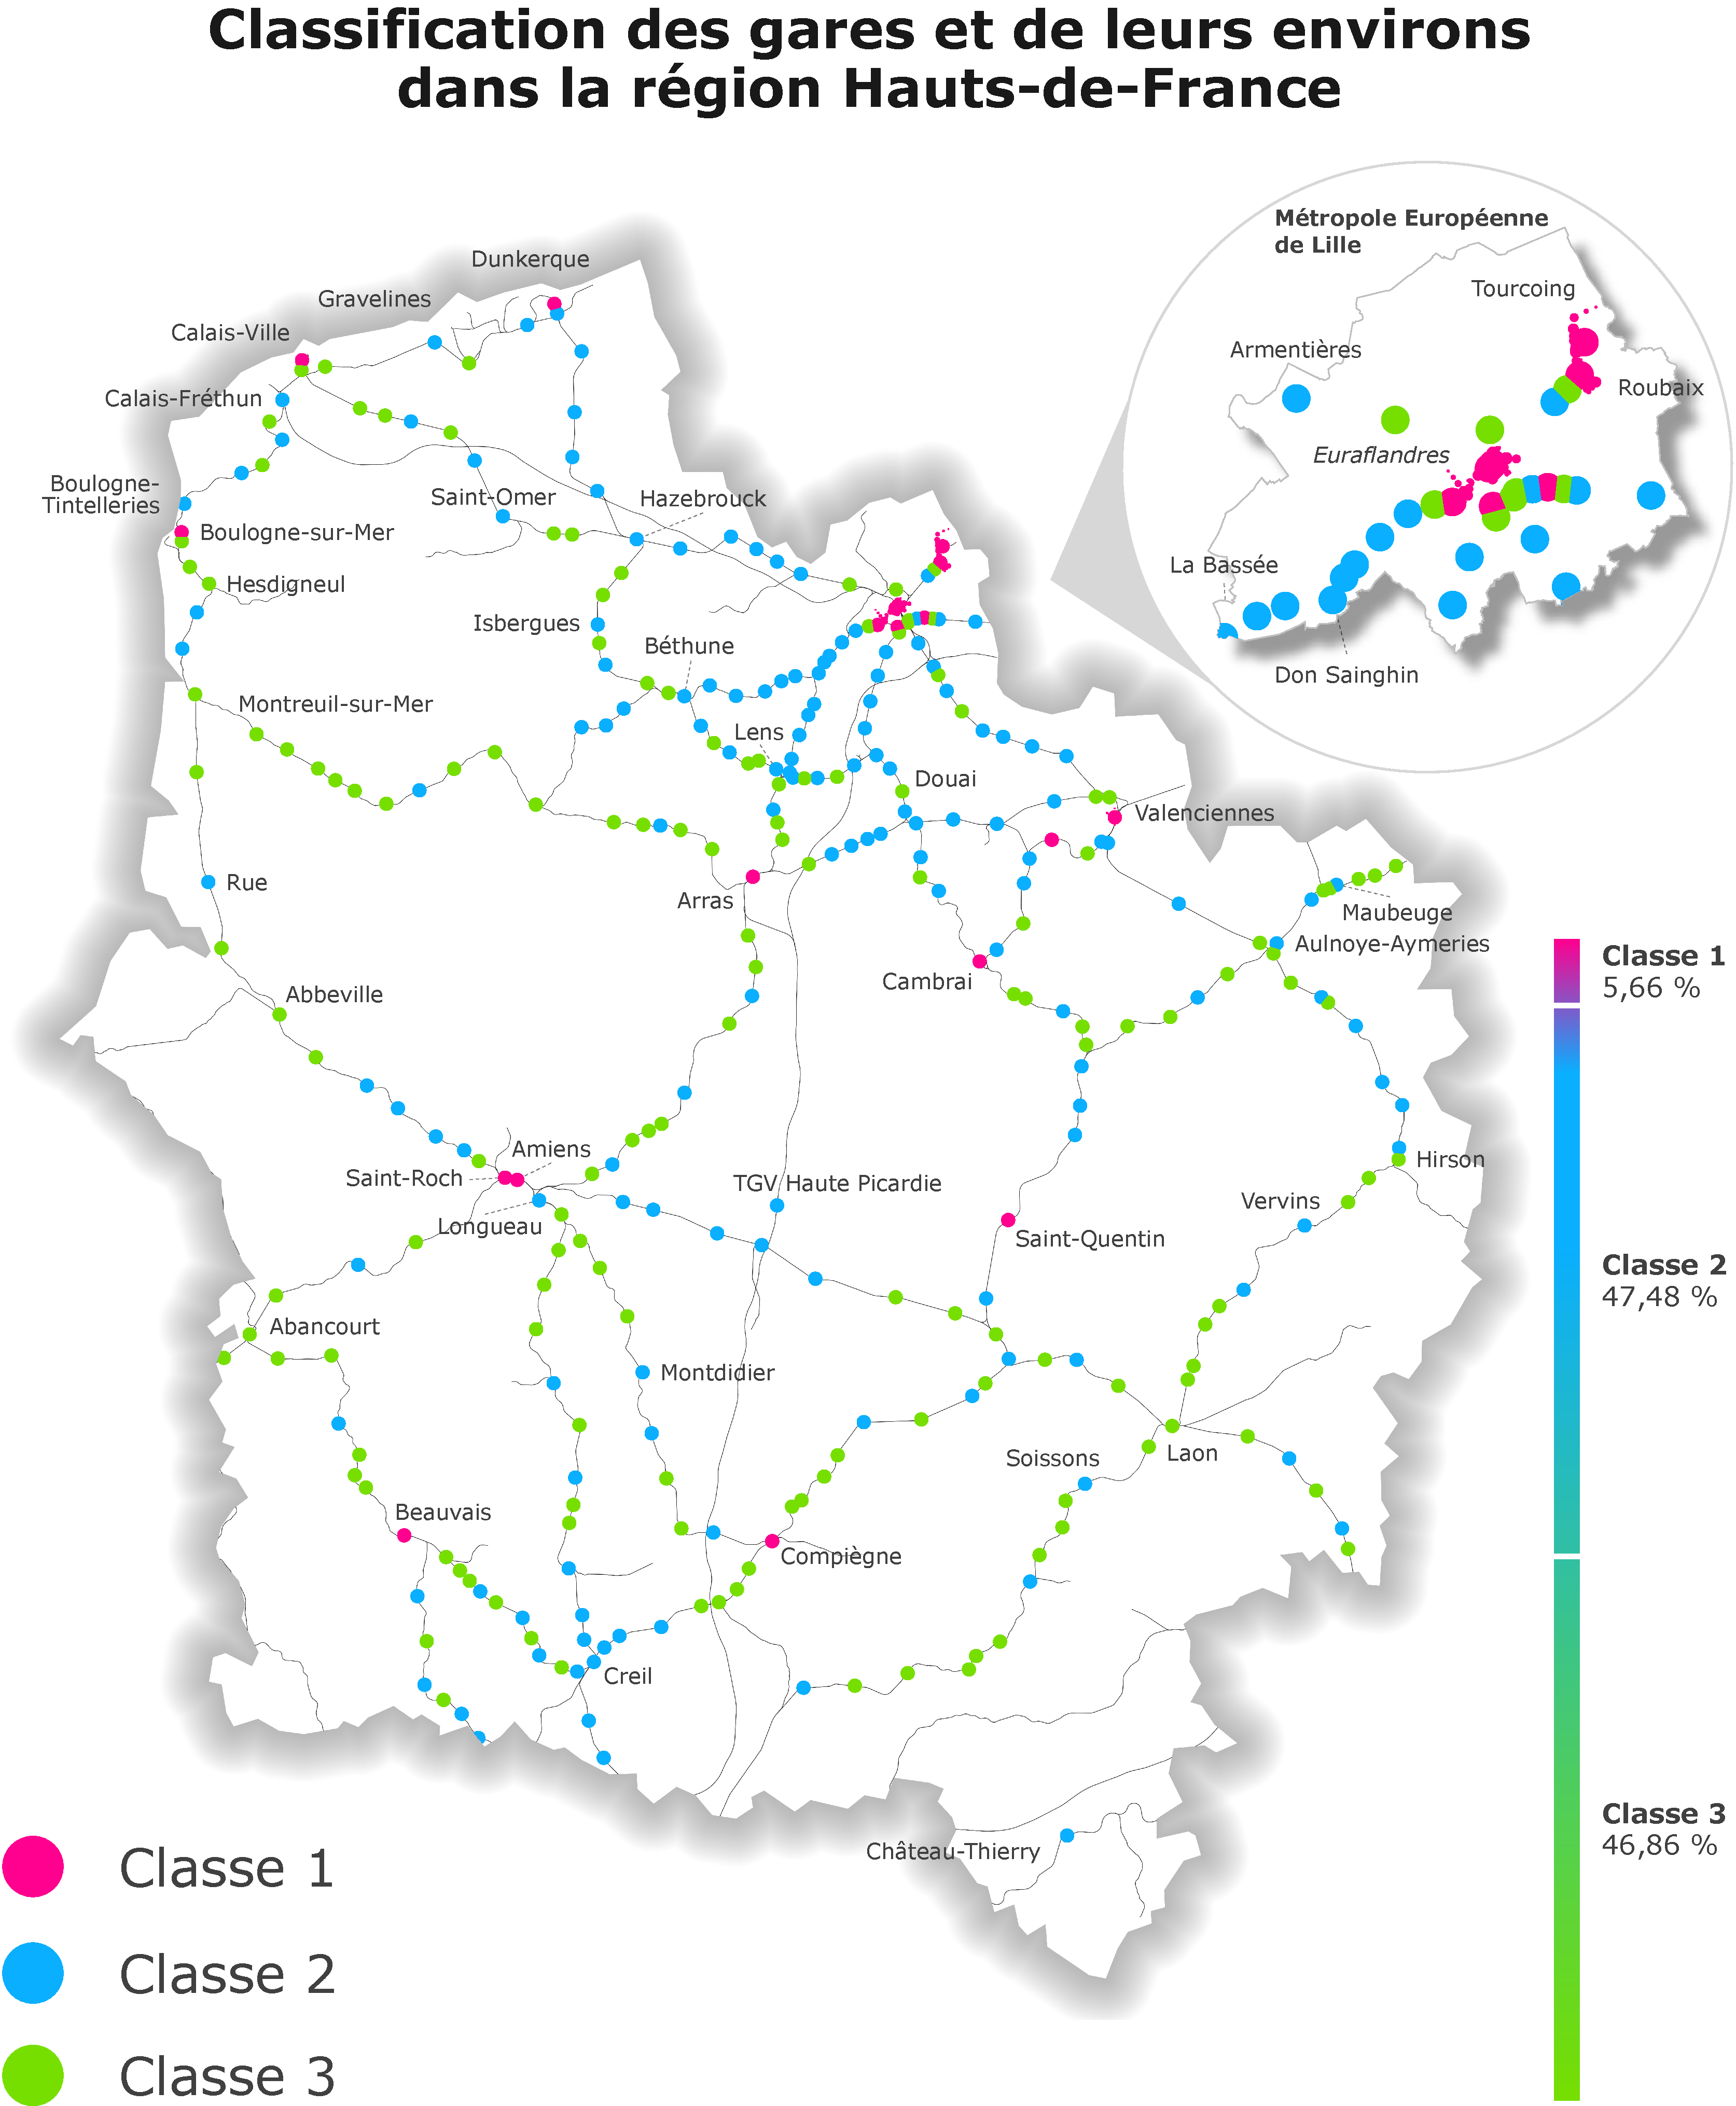
\includegraphics[width=\columnwidth]{figures/policy-brief-carte-classification-compresse.pdf}
    \label{classification-npart}
    \vspace{-0.2cm}
    \begin{flushright}
        \begin{minipage}{1\linewidth}
            \justifying
            \noindent
            \scriptsize{\textcolor{darkgray}{Auteurs~: Dylan Moinse, Ahad Amini Pishro, Alain L'Hostis, Shiquan Zhang, Ndèye Aïta Cissé, Xavier Lehmann, Liu Yuetong, Hu Qixiao, Olivier Theureaux et Heythem Adjeroud (2025)}}
        \end{minipage}
    \end{flushright}
\end{center}

    \end{multicols}

    \end{document}